\documentclass[a4paper]{article}

\usepackage[T1]{fontenc}
\usepackage[french]{babel}
\usepackage{ProfLycee}
\useproflyclib{ecritures}
\usepackage{math-vh}
\usepackage{colortbl}
\usepackage{yhmath}
\usepackage{eurosym}
% *** Réglage des headers ***
\fancyhead[L]{1MATHS6 --- Lycée Victor Hugo}
\fancyhead[R]{O. Laurent --- Année 2024--2025}
% *** Réglage des headers ***

\newcommand{\vect}[1]{\overrightarrow{\,\mathstrut#1\,}}
\def\Oijk{$\left(\text{O}~;~\vect{\imath},~\vect{\jmath},~\vect{k}\right)$}
\tikzstyle{block} = [draw, fill=white, rectangle, 
    minimum height=3em, minimum width=6em]

\newif\ifcuboidshade
\newif\ifcuboidemphedge

\tikzset{
  cuboid/.is family,
  cuboid,
  shiftx/.initial=0,
  shifty/.initial=0,
  dimx/.initial=3,
  dimy/.initial=3,
  dimz/.initial=3,
  scale/.initial=1,
  densityx/.initial=1,
  densityy/.initial=1,
  densityz/.initial=1,
  rotation/.initial=0,
  anglex/.initial=0,
  angley/.initial=90,
  anglez/.initial=225,
  scalex/.initial=1,
  scaley/.initial=1,
  scalez/.initial=0.5,
  front/.style={draw=black,fill=white},
  top/.style={draw=black,fill=white},
  right/.style={draw=black,fill=white},
  shade/.is if=cuboidshade,
  shadecolordark/.initial=black,
  shadecolorlight/.initial=white,
  shadeopacity/.initial=0.15,
  shadesamples/.initial=16,
  emphedge/.is if=cuboidemphedge,
  emphstyle/.style={thick},
}

\newcommand{\tikzcuboidkey}[1]{\pgfkeysvalueof{/tikz/cuboid/#1}}

% Commands
\newcommand{\tikzcuboid}[1]{
    \tikzset{cuboid,#1} % Process Keys passed to command
  \pgfmathsetlengthmacro{\vectorxx}{\tikzcuboidkey{scalex}*cos(\tikzcuboidkey{anglex})*28.452756}
  \pgfmathsetlengthmacro{\vectorxy}{\tikzcuboidkey{scalex}*sin(\tikzcuboidkey{anglex})*28.452756}
  \pgfmathsetlengthmacro{\vectoryx}{\tikzcuboidkey{scaley}*cos(\tikzcuboidkey{angley})*28.452756}
  \pgfmathsetlengthmacro{\vectoryy}{\tikzcuboidkey{scaley}*sin(\tikzcuboidkey{angley})*28.452756}
  \pgfmathsetlengthmacro{\vectorzx}{\tikzcuboidkey{scalez}*cos(\tikzcuboidkey{anglez})*28.452756}
  \pgfmathsetlengthmacro{\vectorzy}{\tikzcuboidkey{scalez}*sin(\tikzcuboidkey{anglez})*28.452756}
  \begin{scope}[xshift=\tikzcuboidkey{shiftx}, yshift=\tikzcuboidkey{shifty}, scale=\tikzcuboidkey{scale}, rotate=\tikzcuboidkey{rotation}, x={(\vectorxx,\vectorxy)}, y={(\vectoryx,\vectoryy)}, z={(\vectorzx,\vectorzy)}]
    \pgfmathsetmacro{\steppingx}{1/\tikzcuboidkey{densityx}}
  \pgfmathsetmacro{\steppingy}{1/\tikzcuboidkey{densityy}}
  \pgfmathsetmacro{\steppingz}{1/\tikzcuboidkey{densityz}}
  \newcommand{\dimx}{\tikzcuboidkey{dimx}}
  \newcommand{\dimy}{\tikzcuboidkey{dimy}}
  \newcommand{\dimz}{\tikzcuboidkey{dimz}}
  \pgfmathsetmacro{\secondx}{2*\steppingx}
  \pgfmathsetmacro{\secondy}{2*\steppingy}
  \pgfmathsetmacro{\secondz}{2*\steppingz}
  \foreach \x in {\steppingx,\secondx,...,\dimx}
  { \foreach \y in {\steppingy,\secondy,...,\dimy}
    {   \pgfmathsetmacro{\lowx}{(\x-\steppingx)}
      \pgfmathsetmacro{\lowy}{(\y-\steppingy)}
      \filldraw[cuboid/front] (\lowx,\lowy,\dimz) -- (\lowx,\y,\dimz) -- (\x,\y,\dimz) -- (\x,\lowy,\dimz) -- cycle;
    }
    }
  \foreach \x in {\steppingx,\secondx,...,\dimx}
  { \foreach \z in {\steppingz,\secondz,...,\dimz}
    {   \pgfmathsetmacro{\lowx}{(\x-\steppingx)}
      \pgfmathsetmacro{\lowz}{(\z-\steppingz)}
      \filldraw[cuboid/top] (\lowx,\dimy,\lowz) -- (\lowx,\dimy,\z) -- (\x,\dimy,\z) -- (\x,\dimy,\lowz) -- cycle;
        }
    }
    \foreach \y in {\steppingy,\secondy,...,\dimy}
  { \foreach \z in {\steppingz,\secondz,...,\dimz}
    {   \pgfmathsetmacro{\lowy}{(\y-\steppingy)}
      \pgfmathsetmacro{\lowz}{(\z-\steppingz)}
      \filldraw[cuboid/right] (\dimx,\lowy,\lowz) -- (\dimx,\lowy,\z) -- (\dimx,\y,\z) -- (\dimx,\y,\lowz) -- cycle;
    }
  }
  \ifcuboidemphedge
    \draw[cuboid/emphstyle] (0,\dimy,0) -- (\dimx,\dimy,0) -- (\dimx,\dimy,\dimz) -- (0,\dimy,\dimz) -- cycle;%
    \draw[cuboid/emphstyle] (0,\dimy,\dimz) -- (0,0,\dimz) -- (\dimx,0,\dimz) -- (\dimx,\dimy,\dimz);%
    \draw[cuboid/emphstyle] (\dimx,\dimy,0) -- (\dimx,0,0) -- (\dimx,0,\dimz);%
    \fi

    \ifcuboidshade
    \pgfmathsetmacro{\cstepx}{\dimx/\tikzcuboidkey{shadesamples}}
    \pgfmathsetmacro{\cstepy}{\dimy/\tikzcuboidkey{shadesamples}}
    \pgfmathsetmacro{\cstepz}{\dimz/\tikzcuboidkey{shadesamples}}
    \foreach \s in {1,...,\tikzcuboidkey{shadesamples}}
    {   \pgfmathsetmacro{\lows}{\s-1}
        \pgfmathsetmacro{\cpercent}{(\lows)/(\tikzcuboidkey{shadesamples}-1)*100}
        \fill[opacity=\tikzcuboidkey{shadeopacity},color=\tikzcuboidkey{shadecolorlight}!\cpercent!\tikzcuboidkey{shadecolordark}] (0,\s*\cstepy,\dimz) -- (\s*\cstepx,\s*\cstepy,\dimz) -- (\s*\cstepx,0,\dimz) -- (\lows*\cstepx,0,\dimz) -- (\lows*\cstepx,\lows*\cstepy,\dimz) -- (0,\lows*\cstepy,\dimz) -- cycle;
        \fill[opacity=\tikzcuboidkey{shadeopacity},color=\tikzcuboidkey{shadecolorlight}!\cpercent!\tikzcuboidkey{shadecolordark}] (0,\dimy,\s*\cstepz) -- (\s*\cstepx,\dimy,\s*\cstepz) -- (\s*\cstepx,\dimy,0) -- (\lows*\cstepx,\dimy,0) -- (\lows*\cstepx,\dimy,\lows*\cstepz) -- (0,\dimy,\lows*\cstepz) -- cycle;
        \fill[opacity=\tikzcuboidkey{shadeopacity},color=\tikzcuboidkey{shadecolorlight}!\cpercent!\tikzcuboidkey{shadecolordark}] (\dimx,0,\s*\cstepz) -- (\dimx,\s*\cstepy,\s*\cstepz) -- (\dimx,\s*\cstepy,0) -- (\dimx,\lows*\cstepy,0) -- (\dimx,\lows*\cstepy,\lows*\cstepz) -- (\dimx,0,\lows*\cstepz) -- cycle;
    }
    \fi

  \end{scope}
}


\begin{document}

\begin{center}
  {\scshape\LARGE Chapitre 6 --- Suites I\par}
  \vspace{0.5cm}
\end{center}


\begin{center}
  {\LARGE Activités\par}
  \vspace{0.5cm}
\end{center}

\begin{activite}{}{}

    À chaque étape, on construit un cube formé de petits cubes.
    \begin{center}
      \begin{tikzpicture}[scale=0.5]
            \draw (0,3) node[black]{\textbf{Étape 1}};
            \draw (4,3) node[black]{\textbf{Étape 2}};
            \draw (10,3) node[black]{\textbf{Étape 3}};
            \draw (18,3) node[black]{\textbf{Étape 4}};
            \tikzcuboid{%
            shiftx=4cm,%
            shifty=8cm,%
            scale=1.00,%
            rotation=0,%
            densityx=1,%
            densityy=1,%
            densityz=1,%
            dimx=2,%
            dimy=2,%
            dimz=2,%
            scalex=1,%
            scaley=1,%
            scalez=1,%
            anglex=-30,%
            angley=90,%
            anglez=210,%
            front/.style={draw=green!50!black,fill=green!50!white},%
            top/.style={draw=green!50!black,fill=green!50!white},%
            right/.style={draw=green!50!black,fill=green!50!white},%
            emphedge,%
            emphstyle/.style={line width=1pt, green!50!black},
            shade,%
            shadesamples=64,%
            shadeopacity=0.15,%
            }
            \tikzcuboid{%
            shiftx=10cm,%
            shifty=8cm,%
            scale=1.00,%
            rotation=0,%
            densityx=1,%
            densityy=1,%
            densityz=1,%
            dimx=3,%
            dimy=3,%
            dimz=3,%
            scalex=1,%
            scaley=1,%
            scalez=1,%
            anglex=-30,%
            angley=90,%
            anglez=210,%
            front/.style={draw=green!50!black,fill=green!50!white},%
            top/.style={draw=green!50!black,fill=green!50!white},%
            right/.style={draw=green!50!black,fill=green!50!white},%
            emphedge,%
            emphstyle/.style={line width=1pt, green!50!black},
            shade,%
            shadesamples=64,%
            shadeopacity=0.15,%
            }
            \tikzcuboid{%
            shiftx=18cm,%
            shifty=8cm,%
            scale=1.00,%
            rotation=0,%
            densityx=1,%
            densityy=1,%
            densityz=1,%
            dimx=4,%
            dimy=4,%
            dimz=4,%
            scalex=1,%
            scaley=1,%
            scalez=1,%
            anglex=-30,%
            angley=90,%
            anglez=210,%
            front/.style={draw=green!50!black,fill=green!50!white},%
            top/.style={draw=green!50!black,fill=green!50!white},%
            right/.style={draw=green!50!black,fill=green!50!white},%
            emphedge,%
            emphstyle/.style={line width=1pt, green!50!black},
            shade,%
            shadesamples=64,%
            shadeopacity=0.15,%
            }
            \tikzcuboid{%
            shiftx=0cm,%
            shifty=8cm,%
            scale=0.50,%
            rotation=0,%
            densityx=2,%
            densityy=2,%
            densityz=2,%
            dimx=2,%
            dimy=2,%
            dimz=2,%
            scalex=1,%
            scaley=1,%
            scalez=1,%
            anglex=-30,%
            angley=90,%
            anglez=210,%
            front/.style={draw=green!50!white,fill=green!50!white},%
            top/.style={draw=green!50!white,fill=green!50!white},%
            right/.style={draw=green!50!white,fill=green!50!white},%
            emphedge,%
            emphstyle/.style={line width=1pt, green!50!black},
            shade,%
            shadesamples=64,%
            shadeopacity=0.15,%
            }
      \end{tikzpicture}
    \end{center}
  
  \begin{enumerate}
    \item
    \begin{enumerate}
      \item Combien de petits cubes sont utilisés pour les différentes étapes?
      \vspace{2cm}
      \item Combien de petits cubes sont utilisés pour l'étape 10? Pour l'étape 25?
      \vspace{2cm}
      \item On note $c_1$ le nombre de petits cubes à l'étape 1, $c_2$ le nombre de petits cubes à l'étape 2, etc.\\
      Ecrire avec cette notation les résultats des précédentes questions.
      \vspace{2cm}
  
    \end{enumerate}
     \item On considère désormais que le petit cube unique est l'étape 0.
      \begin{enumerate}
       \item Combien de cubes sont utilisés pour l'étape 4 ?
      \vspace{1cm}
      \item On note $a_0$ le nombres de cubes à l'étape $0$, etc. Donner les valeurs de $a_4$, $a_{10}$, et $a_{25}$.
        \vspace{2cm}
    \end{enumerate}
  
    \item (Pour les plus rapides***): A l'étape 10, déterminer le nombre de segments unitaires visibles sur le cube.
    \vspace{2cm}
  
  \end{enumerate}
  
\end{activite}


\pagebreak

\begin{activite}{}{}
		On considère le tableau suivant:
		\begin{center}
			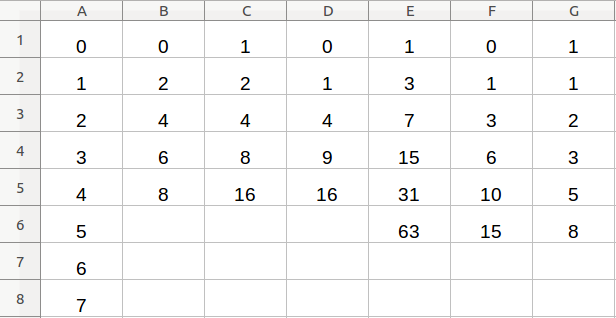
\includegraphics[width=13cm]{img/AC2-Tableau.png}
		\end{center}

	\begin{enumerate}
		\item Complétez les colonnes de la manière qui vous semble la plus logique.
		\item Imaginons que le tableau s'étende vers le bas, quels nombres y aura-t-il dans
		les case $B50$, $C15$ et $D25$?
		\vspace{4cm}
		\item En utilisant un tableur, quelles formules doit-on écrire (en B6, C6, D6, E7, F7, G7) si on désire étendre vers le bas
		le tableau?
    \vspace{3cm}
	\end{enumerate}
\end{activite}

\pagebreak

\section{Notion de suite}
\subsection{Définition}
\begin{definition}{}{}
	Une suite $u$ de nombre réels est une fonction définie dans l'ensemble des entiers naturels:
  \begin{displaymath}
    u:
    \left|
      \begin{array}{rcl}
        \N & \longrightarrow &\R \\
        n & \longmapsto & u(n) \\
      \end{array}
    \right.
    \end{displaymath}

  Le terme $u(n)$ c'est-à-dire l'image par $u$ de $n$, est le plus souvent noté $u_n$.

\end{definition}

\begin{example}{}{}
	La liste des carrés des nombres entiers est une suite: ses premiers termes sont $1$, $4$, $9$, $16$, ...\\
	On peut noter $u_0$ le premier terme, $u_1$ le deuxième, etc.\\
	On a ainsi $u_0=\ldots$, $u_1=\ldots$, $u_2=\ldots$, et plus généralement $u_n=\ldots$.
\end{example}

\begin{vocabulaire}{}{}
		La suite $u_0$, $u_1$, etc. est notée $(u_n)$. On dit qu'elle est définie sur $\N$.\\
		$u_n$ est le \underline{terme général} ou \underline{terme d'indice $n$} de la suite $(u_n)$.
\end{vocabulaire}

\subsection{Mode de génération d'une suite}
	\subsubsection{Suite définie de façon explicite}


		\begin{example}{}{}
			Soit $(u_n)$ la suite définie par $u_n=-n^2+n-2$. Elle est alors définie par l'expression du terme général en fonction de $n$.

			Dans ce cas, on sait calculer directement n'importe quel terme de la suite:
		  \begin{center}
        \renewcommand{\arraystretch}{2.0}
        \begin{tabular}{|*{11}{C{1.2cm}|}}
            \hline
            $n$ & 0 & 1 & 2 & 3 & 4 & 5 & 6 & 7 & 8 & 9 \\
            \hline
            $u_n$ & & & & & & & & & & \\
            \hline
        \end{tabular}
      \end{center}
		\end{example}
		\begin{remark}{}{}
			Le terme général est alors de la forme $u_n=f(n)$.
      
      On peut donc utiliser le tableau de valeurs de la calculatrice pour calculer les termes de la suite.
		\end{remark}


		\subsubsection{Suite définie par récurrence}
		\begin{example}{}{}
			On peut également construire des suites à l'aide d'un procédé. 
      
      On définit par exemple la suite $(v_n)$ de premier terme $v_0=5$
      et dont le terme suivant est obtenu en multipliant par 2 le terme précédent est en ajoutant $3$.\\

      \begin{center}
        \begin{tikzpicture}[node distance=3cm, auto]
          \node (start) [block] {Entrée};
          \node (mult) [block, right of=start] {Multiplier par 2};
          \node (add) [block, right of=mult] {Ajouter 3};
          \node (end) [block, right of=add] {Sortie};

          \draw [black, ->, very thick] (start) -- (mult);
          \draw [black, ->, very thick] (mult) -- (add);
          \draw [black, ->, very thick] (add) -- (end);
        \end{tikzpicture}
      \end{center}

			On a alors $v_0=5$, $v_1=2\times v_0 +3=13$, $v_2=2\times v_1+3=29$, et plus généralement $v_{n+1}=2v_n+3$.
		\end{example}

		\begin{definition}{}{}
			On définit une suite par récurrence en donnant deux informations:
			\begin{itemize}[label=\textbullet]
				\item son premier terme
				\item une relation qui permet de calculer, à partir de chaque terme, le terme suivant, c'est-à-dire une relation du type $u_{n+1}=f(u_n)$.
			\end{itemize}
			Cette relation est appelée \underline{relation de récurrence}.
		\end{definition}

		\begin{example}{}{}
			Dans l'exemple précédent, on note alors la suite $(v_n)$ de la façon suivante:
			$$\begin{cases}
				v_0 &=5\\
				v_{n+1} &=2v_n+3\\
		\end{cases}$$
		\end{example}

    \pagebreak
    \subsubsection{Suite définie par un algorithme}
    On peut définir une suite par son premier terme et des instructions dans une boucle \textquote{Pour} qui permet de calculer les termes suivants.

    \begin{example}{}{}
      \begin{PseudoCode}{} 
U = 4
Pour i variant de 1 à n Faire
  U = 2*U+1
FinPour
        \end{PseudoCode}
        $U$ représente le terme initial de la suite $u_0$, puis on calcule $u_1=2u_0+1$, et ainsi de suite.

        Après les $N$ étapes, $U$ correspond au terme $u_n$.
    \end{example}


    \subsubsection{Suite définie par des motifs géométriques}

    La suite $(u_n)$ peut être définie comme une quantité géométrique dans une figure ou un motif particulier se 
    répète.

    \begin{example}{}{}
    A l'aide des motifs suivants:
    \begin{center}
    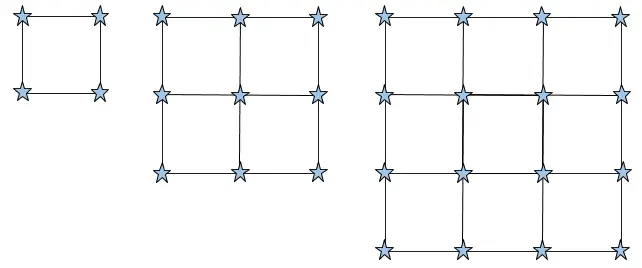
\includegraphics[width=10cm]{img/geometrie1.png}
    \end{center}
    On définit une suite $(u_n)$ qui définit le nombre de segments contenus dans le motif à l'étape $n$.

    Ainsi, $u_0=4$, $u_1=12$, $u_2=24$, avec plus généralement $u_n=$
    \end{example}


    \begin{methode}{Calculer les termes d'une suite définie par récurrence à l'aide de la calculatrice}{}

    \begin{tabular}{ccc}
      \MethodeQRCodeMini{https://www.youtube.com/watch?v=_EOfvb6FsS0}{\textbf{Numworks}}&
      \MethodeQRCodeMini{https://www.youtube.com/watch?v=D5OAi2_h_bw}{\textbf{TI-83}}&
      \MethodeQRCodeMini{https://www.youtube.com/watch?v=x_lNORNjrqQ}{\textbf{Casio}}
    \end{tabular}
    

    \end{methode}
\begin{exercices}{}{}
  13--20 p.84, 40--49 p.86, 50--51 p.87, 55--58 p.87, 60--61 p.87
\end{exercices}


\pagebreak

\section{Sens de variation d'une suite}
\begin{definition}{}{}
  Une suite $(u_n)$ est dite :
  
  \begin{itemize}
    \item strictement croissante si pour tout $n\in\N$: $u_{n+1} > u_n$.
    \item strictement décroissante si pour tout $n\in\N$: $u_{n+1} <  u_n$
    \item constante si pour tout $n\in\N$: $u_{n+1}= u_n$
    \item monotone si elle est soit croissante, soit décroissante, soit constante.
  \end{itemize}
\end{definition}

\begin{example}{}{}
  Dans l'exemple précédent, la suite $(u_n)$ définie par $u_n=\sqrt{n}$ est strictement croissante.\\
  En effet, pour tout entier naturel $n$, on a: $n+1>n$ et puisque la fonction racine carrée est strictement
  croissante sur $[0;+\infty[$, on en déduit que $\sqrt{n+1}>\sqrt{n}$, soit $u_{n+1}>u_n$.
\end{example}

\begin{methode}{\'Etude du sens de variation d'une suite}{}
  Pour étudier le sens de variation d'une suite $(u_n)$, on étudie \textbf{le signe de $u_{n+1}-u_{n}$}.

  Exemple : Soit $(u_n)$ la suite définie par $u_n=\dfrac{2n-4}{n+1}$. On a alors:
  
\vspace{.3cm}
  $\forall n \in \N$, $u_{n+1}-u_n=$

  \vspace{5cm}

\end{methode}


\begin{methode}{\'Etude du sens de variation d'une suite - cas des suites positives}{}
  Pour étudier le sens de variation d'une suite $(u_n)$ pour laquelle $u_n > 0$ pour tout entier $n$,
  on peut calculer \textbf{le rapport $\dfrac{u_{n+1}}{u_{n}}$}.

  Exemple : Soit $(u_n)$ la suite définie par $u_n=\dfrac{3^{4n}}{4^{3n}}$. Pour tout entier $n$, on a bien $u_n > 0$. 
  
  On a alors:
  
\vspace{.3cm}
  $\forall n \in \N$, $\dfrac{u_{n+1}}{u_n}=$

  \vspace{5cm}

\end{methode}

\begin{exerciceapp}{}{}
Etudier les variations des suites $(u_n)$, $(v_n)$ et $(w_n)$ définies par:
\begin{enumerate}
  \item Pour tout entier naturel $n$, $u_n=\dfrac{3n-2}{2n+4}$.
  \item Pour tout entier naturel $n$, $v_n=0,5^n$.
  \item Pour tout entier naturel $n$, $w_{n+1}=n+w_n$ avec $w_0=-2$.
\end{enumerate}
\end{exerciceapp}


\pagebreak


		\section{Représentation graphique}

    \subsection{Suite explicite}
		\begin{definition}{}{}
			Dans un repère du plan, la représentation graphique d'une suite $(u_n)$ est l'ensemble des
			points de coordonnées $(n;u_n)$, où $n$ décrit les entiers naturels.
		\end{definition}

		\begin{example}{}{}
			Soit $(u_n)$ la suite définie par $u_n=\sqrt{n}$, définie explicitement.
      Il suffit de connaître la représentation graphique de la fonction $f:x\mapsto \sqrt{x}$ pour obtenir celle de la suite.

			\begin{center}
				\begin{tikzpicture}

				\draw [very thin, gray!30] (-1,-1) grid[step=1] (10,5);
				\foreach \x in {1,...,9} \draw[very thick](\x,0.1) -- (\x,-0.1) node[below]{\x};
				\foreach \y in {1,...,4} \draw[very thick](0.1,\y) -- (-0.1,\y) node[left]{\y};

				\draw[very thick,color=black,->] (0,-1) -- (0,5);
				\draw[very thick,color=black,->] (-1,0) -- (10,0);
				\draw (10,-0.2) node[below]{$n$};

				\draw[red,fill=red] (0,0) circle (.5ex);
				\draw[red,fill=red] (1,1) circle (.5ex);
				\draw[red,fill=red] (2,1.414) circle (.5ex);
				\draw[red,fill=red] (3,1.732) circle (.5ex);
				\draw[red,fill=red] (4,2) circle (.5ex);
				\draw[red,fill=red] (5,2.236) circle (.5ex);
				\draw[red,fill=red] (6,2.45) circle (.5ex);
				\draw[red,fill=red] (7,2.646) circle (.5ex);
				\draw[red,fill=red] (8,2.828) circle (.5ex);
				\draw[red,fill=red] (9,3) circle (.5ex);

				\draw[black, very thick, dashed] (7,2.646) -- (7,0);
				\draw[black, very thick, dashed] (7,2.646) -- (0,2.646) node[left]{$u_7$};

        \draw[blue,domain=0:10,samples=250] plot (\x,{sqrt(\x)}) ;

				\end{tikzpicture}
			\end{center}
		\end{example}

		\begin{remark}{}{}
			La représentation graphique d'une suite est un nuage de points: on ne relie pas les points.
		\end{remark}


    \subsection{Suite définie par récurrence}
    Dans le cas d'une suite définie par récurrence, on ne peut pas tracer directement la représentation graphique de la suite.
    
    On peut cependant déterminer les premiers termes de la suite.

    Pour cela, on trace la représentation graphique de la fonction définie par la relation de récurrence, puis on trace 
    la droite d'équation $y=x$, afin de pouvoir reporter sur l'axe des abscisses les valeurs des premiers termes de la suite.

    Par exemple, soit la suite $(u_n)$ définie par $\begin{dcases}
      u_0 &= 2\\
      u_{n+1} &= \dfrac{1}{4}u_n^2
    \end{dcases}$.

    Après avoir tracé la représentation graphique de la fonction $f:x\mapsto \dfrac{1}{4}x^2$, on peut reporter les premiers termes de la suite.
    
    

    \begin{tabular}{cc}
      \begin{minipage}{10cm}
    
        \begin{center}
          \begin{tikzpicture}[x=1.8cm,y=1.8cm,%unités
          xmin=0,xmax=4.5,xgrille=0.1,xgrilles=1, %axe Ox
          ymin=0,ymax=4.5,ygrille=0.1,ygrilles=1] %axe Oy
              \GrilleTikz
              \AxexTikz[Police=\small]{1,2,3,4}
              \AxeyTikz[Police=\small]{1,2,3,4}
              \AxesTikz
  
  
               \def\f{0.25*\x*\x}
              %toile
              \ToileRecurrence[Fct={\f},No=0,Uno=3.5, Nb=5,DecalLabel=4pt]
              %éléments supplémentaires
  
              \draw[very thick, blue] (3,2.2) node[below right]{$\mathcal{C}_f$};
              \draw[very thick, CouleurVertForet] (4,4) node[below right]{$y=x$};
              \draw[very thick,blue,domain=0:4.24,samples=250] plot (\x,{\f}) ;
              \draw[very thick,CouleurVertForet,domain=0:4.5,samples=2] plot (\x,\x) ;
  
  
          \end{tikzpicture}
      \end{center}
      \end{minipage}
      &
      \begin{minipage}{8cm}
        Pour le tracer à la calculatrice :
        
        \MethodeQRCodeMini{https://www.youtube.com/watch?v=onShyNu0gGw}{\textbf{Numworks}}{}
        \MethodeQRCodeMini{https://www.youtube.com/watch?v=bRlvVs9KZuk}{\textbf{TI-83}}{}
        \MethodeQRCodeMini{https://www.youtube.com/watch?v=9iDvDn3iWqQ}{\textbf{Casio}}{}
        
      \end{minipage}
      \end{tabular}


    \section{Notion de limite d'une suite}

    S'intéresser à la limite d'une suite $(u_n)$, c'est étudier le comportement des termes $u_n$ quand on donne à 
    $n$ des valeurs aussi grandes que l'on veut, ce qui se dit aussi \textquote{quand $n$ tend vers l'infini}.

    \subsection{Limite finie}
On reprend l'exemple précédent de la suite $(u_n)$ définie par $\begin{dcases}
  u_0 &= 2\\
  u_{n+1} &= \dfrac{1}{4}u_n^2
\end{dcases}$.

Graphiquement, on a pu observer que les termes de la suite semblent se rapprocher de $0$. 

On réalise le tableau suivant:
\begin{center}
  \begin{tabular}{|*{5}{C{1.2cm}|}c|c|}
      \hline
      $n$ & 0 & 1 & 2 & 3 & 4 & 9 \\
      \hline
      $u_n$ & 2 & 0,5 & 0,125 & 0,03125 & 0,0078125 & 0,00000762939 \\
      \hline
  \end{tabular}
\end{center}

On peut démontrer que pour tout réel $\varepsilon$ positif, il existe un rang à partir duquel l'écart entre $u_n$ et $0$ est inférieur à $a$, 
c'est-à-dire que pour tout $\varepsilon > 0$, il existe un rang $N$ tel que pour tout $n\geq N$, on a $|u_n-0|<\varepsilon$.

On dit alors que:
\begin{itemize}[label=\textbullet]
  \item la suite $(u_n)$ tend vers $0$ quand $n$ tend vers l'infini, et on note $\lim\limits_{n\to +\infty}u_n=0$.
  \item la suite $(u_n)$ est convergente.
\end{itemize}


    \subsection{Limite infinie}

    On prend l'exemple de la suite $(u_n)$ définie sur $\N$ par $u_n=n^2$.

    \begin{center}

      \begin{tikzpicture}[x=2cm,y=0.5cm,%unités
        xmin=0,xmax=5,xgrille=1,xgrilles=1, %axe Ox
        ymin=0,ymax=20,ygrille=1,ygrilles=1] %axe Oy
            \GrilleTikz
            \AxexTikz[Police=\small]{1,2,3,4}
            \AxeyTikz[Police=\small]{2,4,...,20}
            \AxesTikz

            \draw[color=white, fill=yellow!50] (4,16) rectangle (5,20);
            \draw[very thick, blue] (2,3) node[below right]{$\mathcal{C}_f$};
            \draw[blue,domain=0:4.5,samples=250] plot (\x,{\x*\x}) ;

            \draw[red,fill=red] (0,0) circle (.5ex);
            \draw[red,fill=red] (1,1) circle (.5ex);
            \draw[red,fill=red] (2,4) circle (.5ex);
            \draw[red,fill=red] (3,9) circle (.5ex);
            \draw[red,fill=red] (4,16) circle (.5ex);
           
            \draw[dashed, ForestGreen, very thick] (4,0) -- (4,20) node[below, ForestGreen] {$~$};
           % \draw[ ForestGreen, very thick] (11,0) -- (19.7,0) ;
            \draw[red, thick] (5,16) --  (0,16) node[left, red] {$A$};

        \end{tikzpicture}
    \end{center}

    On peut remarquer à l'aide de la courbe représentative ou de la calculatrice que les termes de la suite augmentent très rapidement.

    On peut démontrer que pour tout réel $A$ positif, il existe un rang à partir duquel $u_n$ est supérieur à $A$, c'est-à-dire que pour tout $A>0$, il existe un rang $N$ tel que pour tout $n\geq N$, on a $u_n>A$.

    On dit alors que:
    
    \begin{itemize}[label=\textbullet]
      \item la suite $(u_n)$ tend vers $+\infty$ quand $n$ tend vers l'infini, et on note $\lim\limits_{n\to +\infty}u_n=+\infty$.
      \item la suite $(u_n)$ est divergente.
    \end{itemize}

    \begin{exercices}{}{}
      63--73 p.88
    \end{exercices}


\end{document}
